\begin{frame}

\frametitle{Introduction: Configuration Management}

\begin{block}{Configuration Management}
Is the process that:
\begin{itemize}
\item Identifies and defines software system elements
\item Manages changes over these elements
\item Registers change requests and the state of elements
\item Verifies the completeness and correctness of the elements
\end{itemize}
\end{block}

Addressed to solve the following problems:
\begin{multicols}{2}

\begin{itemize}
\item Parallel development
\item Version history
\item Unauthored changes
\item Incorrect software construction due to unmatched component versions
\columnbreak
\item Successive requirement changes
\item Software variants

\end{itemize}

\end{multicols}

\end{frame}

\begin{frame}

\frametitle{Introduction: Configuration Management}

\begin{block}{Item Configuration}
Basic unit in terms of configuration management. A Item Configuration is usually a file.
\end{block}

\begin{block}{Item Configuration Version}
Specific instance of a file that differs from other versions at some point.
Examples are:
\begin{itemize}
\item Modified logic function
\item New reqs added to specification document
\end{itemize}
\end{block}

\end{frame}

\begin{frame}

\frametitle{Introduction: Configuration Management}

\begin{block}{Baseline}
Specification or product which have been revised formally and agreed. Further developments are based on this. They are usually related to project milestones.
\end{block}

\begin{multicols}{2}

In the following picture:
\begin{itemize}
\item IC: File A, File C
\item Version IC: A1, A2, C1
\item Baseline: V1, V2, ...
\end{itemize}
 
\columnbreak

\begin{figure}[h]
\centering
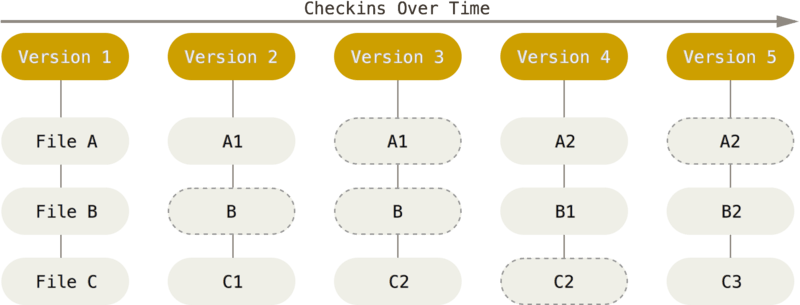
\includegraphics[scale=0.2]{snapshots.png}
\caption{IC evolution over time}
\label{fig:snapshots}
\end{figure}

\end{multicols}
\end{frame}